% TEMPLATE AUTHOR: https://bitbucket.org/m_by/fiit-stu-thesis-template-for-latex
% EDIT: Jozef Gáborík
% OVERLEAF TEMPLATE https://www.overleaf.com/latex/templates/stu-fiit-bachelor-thesis-template-slovak-university-of-technology/pppyykvvhqgq
%
% Customized from OVERLEAF TEMPLATE: Giang Nguyen
% https://www.overleaf.com/read/xmtqfgjhfphj#760c57

% SETTINGS - LATEX
\newcommand{\myFontSize}[0] {11pt}
\newcommand{\mySpacing}[0] {1.1}
\newcommand{\myBibliography}[0] {bib/references}

\documentclass[\myFontSize,a4paper,twoside,openright,english]{book}
% \documentclass[\myFontSize,a4paper,twoside,openright,slovak]{book}

% to change name, title, supervisor etc. go to preamble/preamble.tex
\usepackage[utf8]{inputenc}
\usepackage[T1]{fontenc}
% \usepackage[slovak]{babel}
\usepackage[english]{babel}
\usepackage[a4paper]{geometry}
\usepackage[
    left = \glqq,% 
    right = \grqq,% 
    leftsub = \glq,% 
    rightsub = \grq%
]{dirtytalk}

% SETTINGS - NAMES
\newcommand{\myTitle}[0] {My Thesis title}
\newcommand{\myTitleSK}[0] {My Thesis title SK}
\newcommand{\myName}[0] {(Bc.) František Paradajka}
\newcommand{\mySupervisor}[0] {doc. Ing. Giang Nguyen Thu, PhD.}
\newcommand{\myEvidenceNumber}[0] {FIIT-XXXX-XXXXX}
\newcommand{\myDate}[0] {May 20xx}
\newcommand{\myDateSK}[0] {Máj 20xx}
\newcommand{\myStudyProgram}[0] {Intelligent Software Systems}
\newcommand{\myStudyProgramSK}[0] {Inteligentné softvérové systémy}
\newcommand{\myStudyField}[0] {Computer Science}
\newcommand{\myStudyFieldSK}[0] {Informatika}
\newcommand{\myUniversity}[0] {Slovak University of Technology in Bratislava}
\newcommand{\myUniversitySK}[0] {Slovenská technická univerzita v Bratislave}
\newcommand{\myFaculty}[0] {Faculty of Informatics and Information Technologies}
\newcommand{\myFacultySK}[0] {Fakulta informatiky a informačných technológií}
\newcommand{\myInstitute}[0] {Institute of Informatics, Information Systems and Software Engineering}
\newcommand{\myInstituteSK}[0] {Ústav informatiky, informačných systémov a softvérového inžinierstva}

\usepackage[parfill]{parskip}
\usepackage{enumitem}

\usepackage{graphicx}
\usepackage{float}
\usepackage{longtable}
\usepackage{setspace}

% Spacing
\setstretch{\mySpacing}

\setcounter{secnumdepth}{3}
\setcounter{tocdepth}{3}

\usepackage{tabularx}
\newsavebox\mybox
\usepackage{fancyhdr}
\pagestyle{fancy}
\lhead{\nouppercase{\leftmark}}
\chead{}
\rhead{}
\lfoot{}
\cfoot{\thepage}
\rfoot{}


%style=iso-numeric
%style=authortitle-dw
\usepackage[backend=bibtex,sorting=none,defernums=true]{biblatex}
\defbibheading{references}[Literatúra]{ 
  \chapter*{#1}
  \markboth{#1}{#1}
}
\defbibheading{referencessec}[Literatúra]{ 
  \section*{#1}
  \markboth{#1}{#1}
}
\bibliography{\myBibliography}


% Listing as figure
%\usepackage{libs/minted}
%\usepackage[section]{minted}

\usepackage{listing}

% openright does not work :(
\let\tmp\oddsidemargin
\let\oddsidemargin\evensidemargin
\let\evensidemargin\tmp
\reversemarginpar

\usepackage{lscape}
\usepackage{afterpage}

\usepackage{lipsum}

% Acronyms in automatic way
% \usepackage{acro}[=v2] % default is v3, and causing timeout
% \acsetup{list/template=longtable}

% GN setting begin
% https://tug.org/FontCatalogue/
% \usepackage{mathpazo}           % EN + math font in one
\usepackage{newpxtext}        % slovencina, aby nerobila problem s CRZP
% \usepackage{eulerpx}          % math font for newpxtext
\usepackage{amsfonts, amssymb, amsmath}     % math symboly

% URL without red/blue boxing
\usepackage[hidelinks,unicode]{hyperref}

% Clean the space among items
\usepackage{etoolbox}
\AtBeginEnvironment{itemize}{\setlength\parskip{0pt}}
\AtBeginEnvironment{enumerate}{\setlength\parskip{0pt}}

% include PDF zadanie z AISu (alebo draft PDF zadania z YonBanu)
\usepackage{pdfpages}

% Acronyms/Abbreviations in automatic way
%\usepackage{longtable}
\usepackage{acro}[=v2] % default is v3, and causing Overleaf timeout
% https://www.overleaf.com/learn/latex/Glossaries

%\usepackage[acronym]{glossaries}
% \usepackage{acro}[=v2] % default is v3, and causing Overleaf timeout

%\makeglossaries

\DeclareAcronym{nlp}{   short=NLP,  long=Natural Language Processing,  }
\DeclareAcronym{llm}{   short=LLM,  long=Large Language Model,   }
\DeclareAcronym{ai}{    short=AI,   long=Artificial Intelligence,    }
\DeclareAcronym{ner}{   short=NER,  long=Named Entity Recognition,   }
\DeclareAcronym{lda}{   short=LDA,  long=Latent Dirichlet Allocation,   }
\DeclareAcronym{cnn}{   short=CNN,  long=Convolutional Neural Network,  }
\DeclareAcronym{rnn}{   short=RNN,  long=Recurrent Neural Network,  }
\DeclareAcronym{tp}{    short=TP,   long=True Positive, }
\DeclareAcronym{fp}{    short=FP,   long=False Positive,    }
\DeclareAcronym{fn}{    short=FN,   long=False Negative,    }
\DeclareAcronym{tn}{    short=TN,   long=True Negative, }
\DeclareAcronym{nn}{    short=NN,   long=Neural Network,    }
\DeclareAcronym{ml}{    short=ML,   long=Machine Learning,  }
\DeclareAcronym{lstm}{  short=LSTM, long=Long Short-Term Memory,    }
\DeclareAcronym{gru}{   short=GRU,  long=Gated Recurrent Unit,  }
\DeclareAcronym{crf}{   short=CRF,  long=Conditional Random Field,  }
\DeclareAcronym{nmf}{   short=NMF,  long=Non-negative Matrix Factorization, }
\DeclareAcronym{lsi}{   short=LSI,  long=Latent Semantic Indexing,  }
\DeclareAcronym{bert}{  short=BERT, long=Bidirectional Encoder Representations from Transformers,   }
\DeclareAcronym{svd}{   short=SVD,  long=Single Value Decomposition,    }
\DeclareAcronym{ntm}{   short=NTM,  long=Neural Topic Model,    }
\DeclareAcronym{jsd}{   short=JS divergence,    long=Jensen-Shannon divergence, }
\DeclareAcronym{kld}{   short=KL divergence,    long=Kullback–Leibler divergence, }
% \acsetup{list-style=longtable}

%pseudocode
\usepackage{algorithm}
\usepackage{algpseudocode}

% various
\usepackage{booktabs}       % nicer tables
\usepackage{multirow}
\usepackage{todonotes}      % todo poznamky

\usepackage{pmboxdraw}      % tree drawing
\usepackage{verbatim}       % for verbatim environment and \verbatiminput
\usepackage{sverb}          % for \verbinput
% GN setting end

\begin{document}

% Minted: insert colorful code in the manuscript
% pygmentize -L styles
% \usepackage[cache=false,outputdir=build]{minted}
% \usemintedstyle{autumn}

    
\begin{center}
\thispagestyle{empty}
% {\Large Slovenská technická univerzita v Bratislave}
{\Large \myUniversity}
\par\end{center}{\Large \par}

\begin{center}
% {\Large Fakulta informatiky a informačných technológií}
{\Large \myFaculty}
\par\end{center}{\Large \par}

\smallskip{}

\begin{center}
\myEvidenceNumber
\par\end{center}
\vfill{}

\begin{center}
\textbf{\Large \myName}
\par\end{center}{\Large \par}

\medskip{}


\begin{center}
\textbf{\LARGE \myTitle }
\par\end{center}{\huge \par}

\medskip{}


\begin{center}

% {\Large Bakalárska práca / }
{\Large Master's / Bachelor's Thesis}
\par\end{center}{\Large \par}

\vfill{}

Thesis Supervisor: \mySupervisor

\medskip{}
\myDate

\pagenumbering{roman}

\newpage
\thispagestyle{empty}
\mbox{}
\newpage



\begin{center}
\thispagestyle{empty}
% {\Large Slovenská technická univerzita v Bratislave}
{\Large \myUniversity}
\par\end{center}{\Large \par}

\begin{center}
% {\Large Fakulta informatiky a informačných technológií}
{\Large \myFaculty}
\par\end{center}{\Large \par}

\smallskip{}

\begin{center}
\myEvidenceNumber
\par\end{center}
\vfill{}

\begin{center}
\textbf{\Large \myName}
\par\end{center}{\Large \par}

\medskip{}


\begin{center}
\textbf{\LARGE \myTitle }
\par\end{center}{\huge \par}

\medskip{}


\begin{center}

% {\Large Bakalárska práca / }
{\Large Master's / Bachelor's Thesis}
\par\end{center}{\Large \par}

\vfill{}

\begin{tabbing}
    \=xxxxxxxxxxxxxxxxxxxxi \=\kill
    \> Study Programme:     \> \myStudyProgram  \\
    \> Study Field:         \> \myStudyField  \\
    \> Training Workplace:  \> Bratislava, Slovakia \\
    % \>                      \> \myFaculty     \\
    % \> Training Workplace:  \> Institute of Informatics, \\
    % \>                      \> Information Systems and Software Engineering     \\
    \> Thesis Supervisor:   \> \mySupervisor    
\end{tabbing}
\myDate

% Study programme: \myStudyProgram
% Field of study: \myDegreeCourse
% Training workplace:\\ \myInstitute
% Supervisor: \mySupervisor
% \medskip{}
% \myDate

% Študijný program: \myStudyProgram
% Študijný odbor: \myDegreeCourse
% Miesto vypracovania: \myInstitute
% Vedúci práce: \mySupervisor
% \medskip{}
% \myDate


\newpage
\thispagestyle{empty}
\mbox{}
\newpage

            % Title page
    \newpage
\thispagestyle{empty}
\vspace*{\fill}
Čestne vyhlasujem, že som túto prácu vypracoval samostatne, na základe konzultácií a s použitím uvedenej literatúry.

I declare in my honor that I have prepared this work independently, on the basis of consultations and using the mentioned literature.

\vspace{2cm}
\mbox{}
In Bratislava, \myDate \hfill \myName
\mbox{}

\newpage
\thispagestyle{empty}
\mbox{}
\newpage




\thispagestyle{empty}
\section*{Annotation}
\begin{minipage}[t]{1\columnwidth}%
\myUniversity

\myFaculty

Study Programme: \myStudyProgram

Study Field: \myStudyField\\

Author: \myName

Master's Thesis: \myTitle

Thesis Supervisor: \mySupervisor

\myDate%
\end{minipage}

\bigskip{}
\lipsum[3]

\textbf{Keywords:} 3-5 keywords

\newpage{}
\thispagestyle{empty}

% \newpage
% \thispagestyle{empty}
% \mbox{}
% \newpage




\thispagestyle{empty}
\section*{Anotácia}

\begin{minipage}[t]{1\columnwidth}%
\myUniversitySK

\myFacultySK

Študijný program: \myStudyProgramSK

Študijný odbor:	\myStudyFieldSK\\

Autor: \myName

Diplomová práca: \myTitle

Vedúci diplomového projektu: \mySupervisor

\myDateSK
\end{minipage}

\bigskip{}
\lipsum[3]

\textbf{Oblasť problematiky:} 3-5 kľúčových slov

\newpage{}
\thispagestyle{empty}\medskip{}

% \newpage
% \thispagestyle{empty}
% \mbox{}
% \newpage


\newpage
\thispagestyle{empty}
{\center{BP2, DP3: sem vložte finalne a podpisane zadanie: PDF z AISu}}\\
{\center{BP1, DP1, DP2: sem vložte navrh zadania: PDF z YonBanu}}

% \includepdf[pages=-]{assets/zadanie.pdf}


\newpage
\thispagestyle{empty}
\mbox{}
\newpage

       % Annotation
    \thispagestyle{empty}
% \section*{Poďakovanie}
\section*{Acknowledgements / Poďakovanie}

The acknowledgments and the people to thank go here, don't forget to include your project advisor\ldots

I also thank my family and friends who supported me during the writing of this thesis.


\newpage
\thispagestyle{empty}
\mbox{}
\newpage % Acknowledgements

% Table of contents (TOC)
% \setcounter{tocdepth}{2}          % show max 2+1=3 levels in TOC
    \tableofcontents{}

% References segment
    \begin{refsegment}
        \chapter{Introduction}
\label{chapter:intro}

\pagenumbering{arabic}


%\section{Background and Importance} Without sections.
%\label{sec:background-and-importance}

Relevance of modern applications such as traffic management, law enforcement, toll collection, and smart parking solution.

The Growing need for efficient and cost-effective LPR systems, emphasizing the advantages of deploying them on edge
devices like Raspberry Pi, including reduced latency, enhanced privacy, and lower operational costs compared to cloud-based systems.
        % DP, PhD level
\chapter{Objectives and Methodology}
\label{chapter:objectives-and-methodology}
\label{sec:objectives}

Vybrané ciele pre navrhnuté riešenie alebo špecifikácia požiadaviek (funkčné a nefunkčné požiadavky) na naimplementovaný softvérový produkt.

\begin{itemize}
    \item povinne pre DP a DiZP, ale aj BP môže
    \item max 2 pages for the whole chapter.
\end{itemize}

As presented in Chapter~\ref{chapter:sota}, the area of... is wide with many interesting unsolved problems. Therefore, the goals of this thesis are focused on selected objectives (maximum 3 objective) to... as follows:

\begin{itemize}
    \item Develop a robust LPR system capable of functioning under diverse weather conditions.
    \item Use low-resolution cameras to minimize hardware costs without compromising recognition accuracy.
    \item Implement the solution to run autonomously on a Raspberry Pi, ensuring real-time processing and edge computing capabilities.
\end{itemize}


\section{Methodology}
\label{sec:methodology}

The following steps have been chosen for the design and development of ...

\begin{itemize}
    \item Step 1:
    \item Step 2:
    \item ...
    \item Step n:
\end{itemize}

These steps are commitments to each other in the context of ... of the work.
=======


%\section{Objectives}
%\label{sec:objectives}
%
%Vybrané ciele pre navrhnuté riešenie alebo špecifikácia požiadaviek (funkčné a nefunkčné požiadavky) na naimplementovaný softvérový produkt.
%
%\begin{itemize}
%    \item povinne pre DP a DiZP, ale aj BP môže
%    \item max 2 pages for the whole chapter.
%\end{itemize}
%
%As presented in Chapter~\ref{chapter:sota}, the area of... is wide with many interesting unsolved problems. Therefore, the goals of this thesis are focused on selected objectives (maximum 3 objective) to... as follows:
%
%\begin{itemize}
%    \item Develop a robust LPR system capable of functioning under diverse weather conditions.
%    \item Use low-resolution cameras to minimize hardware costs without compromising recognition accuracy.
%    \item Implement the solution to run autonomously on a Raspberry Pi, ensuring real-time processing and edge computing capabilities.
%\end{itemize}
%
%
%\section{Methodology}
%\label{sec:methodology}
%
%The following steps have been chosen for the design and development of ...
%
%\begin{itemize}
%    \item Step 1:
%    \item Step 2:
%    \item ...
%    \item Step n:
%\end{itemize}
%
%These steps are commitments to each other in the context of ... of the work.
>>>>>>> b921ed1 (sync)

        \chapter{Problem Breakdown}
\label{chapter:problem-breakdown}

\pagenumbering{arabic}


\section{Overview and Limitations of Existing Systems}
\label{sec:overview-and-limitations-of-existing-systems}


\section{Edge AI and its Advantages}
\label{sec:edge-ai-and-its-advantages}


\section{Unified Solution}
\label{sec:proposed-unified-solution}
        \chapter{Challenges}
\label{ch:challenges}


\section{Common Image Defects}
\label{sec:common-image-defects}

\subsection{Blurriness}
\label{subsec:blurriness}

\subsection{Noise}
\label{subsec:noise}

\subsection{Occlusion}
\label{subsec:occlusion}

\subsection{Distortion}
\label{subsec:distortion}

\subsection{Low Resolution}
\label{subsec:low-resolution}


\section{Composition of distortion effects}
\label{sec:composition-of-distortion-effects}


\section{Solving for low-level Devices}
\label{sec:solving-for-low-level-devices}

\subsection{Understanding Resource Constraints on Raspberry Pi and Similar Devices}
\label{subsec:understanding-resource-constraints-on-raspberry-pi-and-similar-devices}


Detail the hardware limitations of Raspberry Pi, such as CPU/GPU performance, memory capacity, and power consumption.

\subsection{Model Optimization}
\label{subsec:model-optimization}


\item Quantization: Reducing the precision of model weights (e.g., from 32-bit to 8-bit) to decrease memory usage
and speed up inference.
\item Pruning: Removing redundant or less significant weights from the model to streamline its structure.
\item Knowledge Distillation: Training a smaller model to replicate the performance of a larger mode,
maintaining accuracy while reducing complexity.

\subsection{Efficient Image Processing Algorithms}
\label{subsec:efficient-image-processing-algorithms}

\subsubsection{Lightweight Super-Resolution}

\item Algorithms like SRCNN or ESPCN that offer super-resolution capabilities with lower computational demands.

\subsubsection{Fast Denoising Techniques}

\item Methods such as Non-Local Means or fast CNN-based denoising models are optimized for real-time performance.

\subsection{Energy Efficiency Considerations}
\label{subsec:energy-efficiency-considerations}


Power management techniques, especially if the Raspberry Pi will be deployed in remote or mobile environments.
Raspberry Pi’s dedicated GPU or external accelerators (e.g., Coral USB Accelerator).


\section{Proposed Solution}
\label{sec:proposed-solution}


        \chapter{Implementation}
\label{chapter:implementation}


\section{Architecture}

\subsection{High-Level Overview}

\begin{itemize}
    \item Diagram illustrating the overall system architecture. Highlight the interaction between the camera,
    Raspberry Pi, image processing modules, OCR component, and any external servers or databases.
\end{itemize}

\subsection{Edge AI Setup}

\begin{itemize}
    \item Detail the specific Raspberry Pi model, along with peripherals (camera module, storage, power
    supply).
    \item How the AI models will be deployed and executed on the device.
\end{itemize}

\subsection{Communication with the Main Server}
\begin{itemize}
    \item Communication protocols and data flow between the Raspberry Pi and a central server.
    Data transmission frequency, security measures, and fallback mechanisms in case of connectivity issues.
\end{itemize}


\section{Model developing and training}

\subsection{Data Collection}

\subsection{Optimization and Training}

\subsection{Model Evaluation}

\subsection{Model Deployment}
        \chapter{Experiments and Evaluation}
\label{chapter:experiments-and-evaluation}

\section{Setup}
\label{sec:exp-setup}

hardware, \\
software, libraries, versioning, \\
virtual environment description and setting, \\
datasets, NDA, \\
etc.


\begin{table}[h!]
    \centering
    \begin{tabular}{lccccc}
    \toprule
Machine & Remote    & Google Colab  & Kaggle    & FIIT Cloud    & Local    \\ 
    \midrule
Python      & 3.9.19        & 3.10.12        & - & -    & 3.10.12        \\
PyTorch     & -             & -              & - & -    & -              \\
TensorFlow  & 2.10          & 2.15           & - & -    & 2.14           \\
GPU (NVIDIA) & RTX xx & Tesla T4 15 GB & Tesla P100 16GB & - & -      \\
CUDA        & 12.2          & 12.2           & - & -    & -              \\
cuDNN       & 8.1.0         & N/A            & - & -    & -              \\
CUDA Toolkit & 11.2.2       & N/A            & - & -    & -              \\ 
RAM    & 32/64 GB        & 51 GB & 30 GB     & 32 GB    & 16 GB         \\
CPU  & 8x cores Intel i7   & -  & Xeon 4x cores & 4x cores & -              \\
Storage    & SSD  & Google Driver  & 73 GB & 128 GB & HDD            \\
    \bottomrule
    \end{tabular}
    \caption{Hardware, software and versioning used for realization}
    \label{table:experiments_environment}
\end{table}


\section{Case Study - Experiment 01}
\section{Case Study - Experiment 02}
\section{Case Study - Experiment 03}



% Summary of the Experiments and Evaluation chapter
\section{Summary}
\label{sec:exp-summary}

Main \emph{key findings} of the work based on the Experiment results
\begin{itemize}
    \item add ...
    \item ...
\end{itemize}

\emph{Discussion} about various considerations based on the experiment results (if needed).


Regarding \emph{limitations} of the work ...
\begin{itemize}
    \item add ...
    \item ...
\end{itemize}

        \chapter{Conclusion}
\label{chapter:conclusion}


% Summary of the whole Thesis work
\section{Summary}
\label{sec:conclusion-summary}

Summary of the whole work including SOTA, design, implementations, experiments, evaluations, key fingdings ... 1 page

\section{Future Work}
\label{sec:conclusion-future-work}

1/2 page

        % Resume: 10% in SK if the Thesis is written in EN
        \addcontentsline{toc}{chapter}{Resumé}
        % 10% v slovenčine pre tých, ktorí majú prácu v EN
\chapter*{Resumé}
\markboth{Resumé}{}
\label{chapter:resume}

Chapter je bez cislovania, pouziva sa len \textbf{boldovanie textu} na zyraznenie useku textu. Bez Figure, Table, atd. ak treba tak odvolava sa na originalne Figure a Table.

10\% v slovenčine pre tých, ktorí majú prácu v EN: preklad
\begin{table}[ht]
    \begin{tabular}{l|l}
    \toprule
        EN & SK \\
    \midrule
        Introduction                            & primerane strucne \\
        SOTA                                    & primerane strucne \\
        SOTA - cast Summary and Starting Points & cele \\
        Objective and Methodology               & cele \\
        Design, Implementation                  & primerane strucne \\
        Experiments and Evaluation              & primerane strucne \\
        Experiments and Evaluation - cast Summary & cele \\
        Conclusion and Future Work              & cele \\
    \bottomrule
    \end{tabular}
    \caption{Resumé}
    \label{tab:Resumé}
\end{table}



        % List of Abbreviations
        \addcontentsline{toc}{chapter}{List of Abbreviations}
        \printacronyms[name=List of Abbreviations, heading=chapter*]
        \markboth{}{}

        % List of Figures
        \addcontentsline{toc}{chapter}{List of Figures}
        % \renewcommand{\listfigurename}{List of figures}
        \listoffigures
        \markboth{}{}

        % List of Tables
        \addcontentsline{toc}{chapter}{List of Tables}
        % \renewcommand{\listtablename}{List of tables}
        \listoftables
        \markboth{}{}

        % List of Algorithms
        % \addcontentsline{toc}{chapter}{List of Algorithms}
        % \listofalgorithms

        % List of Code Samples
        % \clearpage\null
        % \addcontentsline{toc}{chapter}{List of Code Samples}
        % \renewcommand*{\listlistingname}{List of Code Samples}
        % \listoflistings

        % Bibliography
        % \addcontentsline{toc}{chapter}{References}
        \printbibliography[heading=bibintoc,
            title=References,
            segment=\therefsegment,
            resetnumbers=true]
        \markboth{}{}
    \end{refsegment}

% Appendix
    \appendix
    % \setcounter{figure}{0}
% \setcounter{listing}{0}

\pagenumbering{arabic}
\renewcommand*{\thepage}{B-\arabic{page}}



\chapter{Description of Digital Submission \label{cha:cdrom} }

\textbf{Thesis Evidence Number:} \\ \myEvidenceNumber

Obsah elektronického média je väčší ako \texttt{1GB} a preto je odovzdaný vedúcemu záverečnej práce (doc. Ing. Giang Nguyen Thu, PhD.).


\textbf{Name of submitted archive:} \texttt{DP\_MenoPriezvisko.zip}
    % \texttt{BP\_MenoPriezvisko.zip}


The digital part included in the thesis contains the following files:
\begin{itemize}
    \item Ubuntu OS: run in command line \texttt{\$ tree} to get a directory structure as below.
    \item Inspiration from \textit{https://github.com/FIIT-ISA/cookiecutter-data-science}
\end{itemize}


\begin{verbatim}
    ROOT // Root directory.
    │
    ├── flatbuffers // This flatbuffers director
    └── scheme
\end{verbatim}

\begin{figure}[h]
    \begin{centering}
    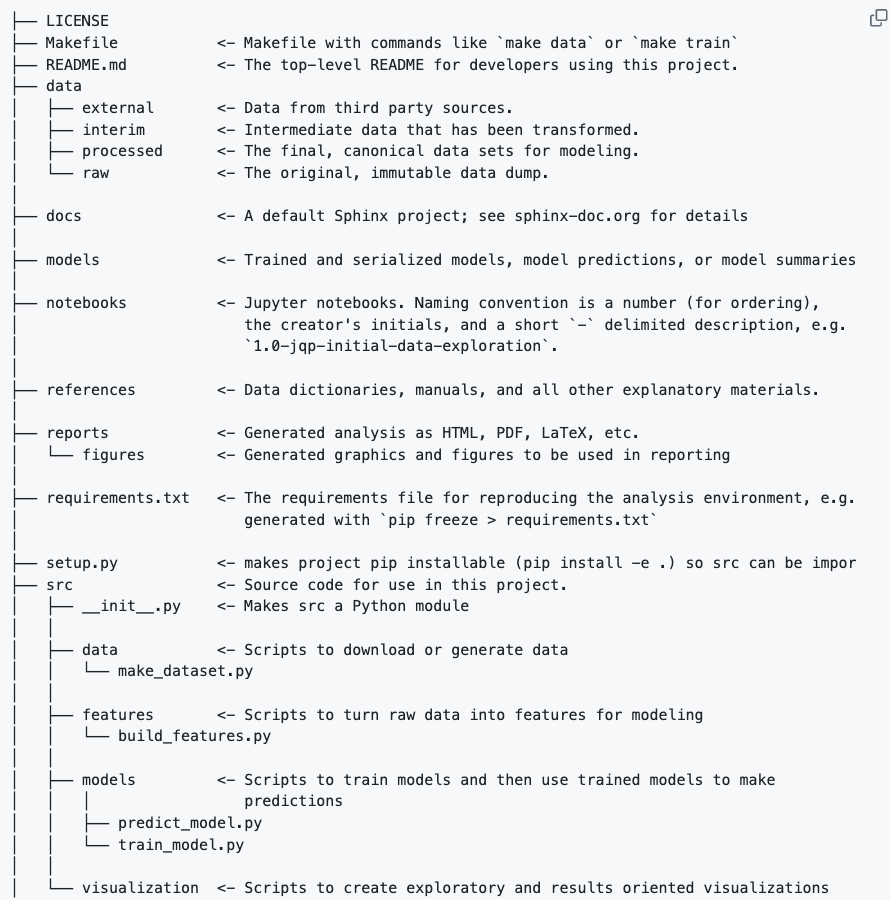
\includegraphics[width=\textwidth]{appendices/zip-file-structure.png}
    \par\end{centering}
\caption{The structure of the ZIP file \label{fig:zip-file-structure}}
\end{figure}



\chapter{Technical Documentation}
\label{chapter:Technical-Documentation}

\section{Installation Manual}
\label{sec:Installation-Manual}

\begin{enumerate}
    \item Clone the project from the Git repository (URL) OR unzip the ZIP file ...
    \item Run \emph{pip install -r requirements.txt} in the root folder of the project
    \item Run \emph{python -m spacy download en} to have the data corpus ...
\end{enumerate}


\section{User Manual / Používateľská príručka}
\label{sec:User-Manual}

\begin{enumerate}
    \item Spustenie programu funguje pomocou hlavného Python súboru \emph{main.py} príkazom \emph{python main.py}. 
    
    \item Po spustení programu sa zobrazí grafické rozhranie programu v ktorom sa dá hneď na hlavnej obrazovke spustiť sumarizácia pre jeden vstupný súbor.

    \item Tlačidlami v hornej časti obrazovky sa dá presúvať medzi funkcionalitami programu ako je viac súborová sumarizácia alebo zobrazovanie článkov. Na týchto obrazovkách sa tlačidlom \emph{Back to main menu} dá vrátiť späť na hlavnú obrazovku.

\end{enumerate}

Screenshot(s) používateľského grafického rozhrania (GUI) ako obrázok (Figure)

(Another variant without GUI: ) The main objective of this work is to ... Several case studies were presented that examine the capabilities of ... to show the feasibility and achievability of ... 
Users in our work are considered to work directly with the code as described in Section~\ref{sec:Installation-Manual}.



\section{Developer Manual}
\label{sec:Developer-Manual}

if needed then add ...
% \setcounter{figure}{0}
\setcounter{listing}{0}

\chapter{First Appendix \label{chapter:appendix-01} }

\begin{refsegment}

% Appendix
% \input{appendices/chapter1}


\end{refsegment}
    % Time schedule
\thispagestyle{empty}

\chapter{Work Schedule}
\label{chapter:Work-Schedule}


\pagenumbering{arabic}
\renewcommand*{\thepage}{B-\arabic{page}}



\section{Work Schedule for BP1/DP1}
\label{sec:Work-Schedule-1st-semester}

\begin{table}[ht]
    \centering
    \begin{tabular}{c|l}
    \toprule
        Week & Plan \\
    \midrule
        1. - 2.     & ... \\
        3. - 4.     & ... \\
        5. - 6.     & ... \\
        7. - 8.     & ... \\
        9. - 10.    & ... \\
        11. - 12.   & ... \\
    \bottomrule
    \end{tabular}
    % \caption{Work Schedule for BP1/DP1}
    \label{tab:dp1}
\end{table}


Some explanation text... (if needed) ... a few sentences

\paragraph{Self-Evaluation of Work Schedule for BP1/DP1:}
Vyjadrenie k plneniu plánu: some text ... one paragraph ... self-evaluation

IAU help: 

(In the best case:) The BP/DP 1 work plan is considered satisfied and successful.



\newpage
\section{Work Schedule for BP2/DP2}
\label{sec:Work-Schedule-2nd-semester}

\begin{table}[ht]
    \centering
    \begin{tabular}{c|l}
    \toprule
        Week & Plan \\
    \midrule
        1. - 2.     & ... \\
        3. - 4.     & ... \\
        5. - 6.     & ... \\
        7. - 8.     & ... \\
        9. - 10.    & ... \\
        11. - 12.   & ... \\
    \bottomrule
    \end{tabular}
    % \caption{Work Schedule for BP2/DP2}
    \label{tab:dp2}
\end{table}

Some explanation text... (if needed) ... a few sentences

\paragraph{Self-Evaluation of Work Schedule for BP2/DP2:}
Vyjadrenie k plneniu plánu: some text ... one paragraph ... self-evaluation

(In the best case:) The BP/DP 2 work plan is considered satisfied and successful.



% \newpage
\section{Work Schedule for DP3}
\label{sec:Work-Schedule-3rd-semester}

\begin{table}[ht]
    \centering
    \begin{tabular}{c|l}
    \toprule
        Week & Plan \\
    \midrule
        1. - 2.     & ... \\
        3. - 4.     & ... \\
        5. - 6.     & ... \\
        7. - 8.     & ... \\
        9. - 10.    & ... \\
        11. - 12.   & ... \\
    \bottomrule
    \end{tabular}
    % \caption{Work Schedule for DP3}
    \label{tab:dp3}
\end{table}

Some explanation text... (if needed) ... a few sentences

\paragraph{Self-Evaluation of Work Schedule for DP3:}
Vyjadrenie k plneniu plánu: some text ... one paragraph ... self-evaluation

(In the best case:) The DP 3 work plan is considered satisfied and successful.

\end{document}
